\documentclass[letterpaper,11pt]{article}
\usepackage[utf8]{inputenc} 
\usepackage{amsmath}
\usepackage{geometry}
\usepackage{graphicx}
\usepackage{tikz}
\usepackage{xcolor}
\usepackage{hyperref}
\usepackage{float} 
\usetikzlibrary{shapes.geometric, arrows, positioning}
\geometry{margin=1in}

\title{\textbf{Research Project Report}}
\author{} 
\date{\today}

\begin{document}

\maketitle
\hrulefill
%\tableofcontents
\vfill

\section{Introduction}
This document will clearly outline the advancement of the research project. Based on the Scrum and sprint methodology, I will update the document every week, including what is new and what is next.
			\begin{center}
            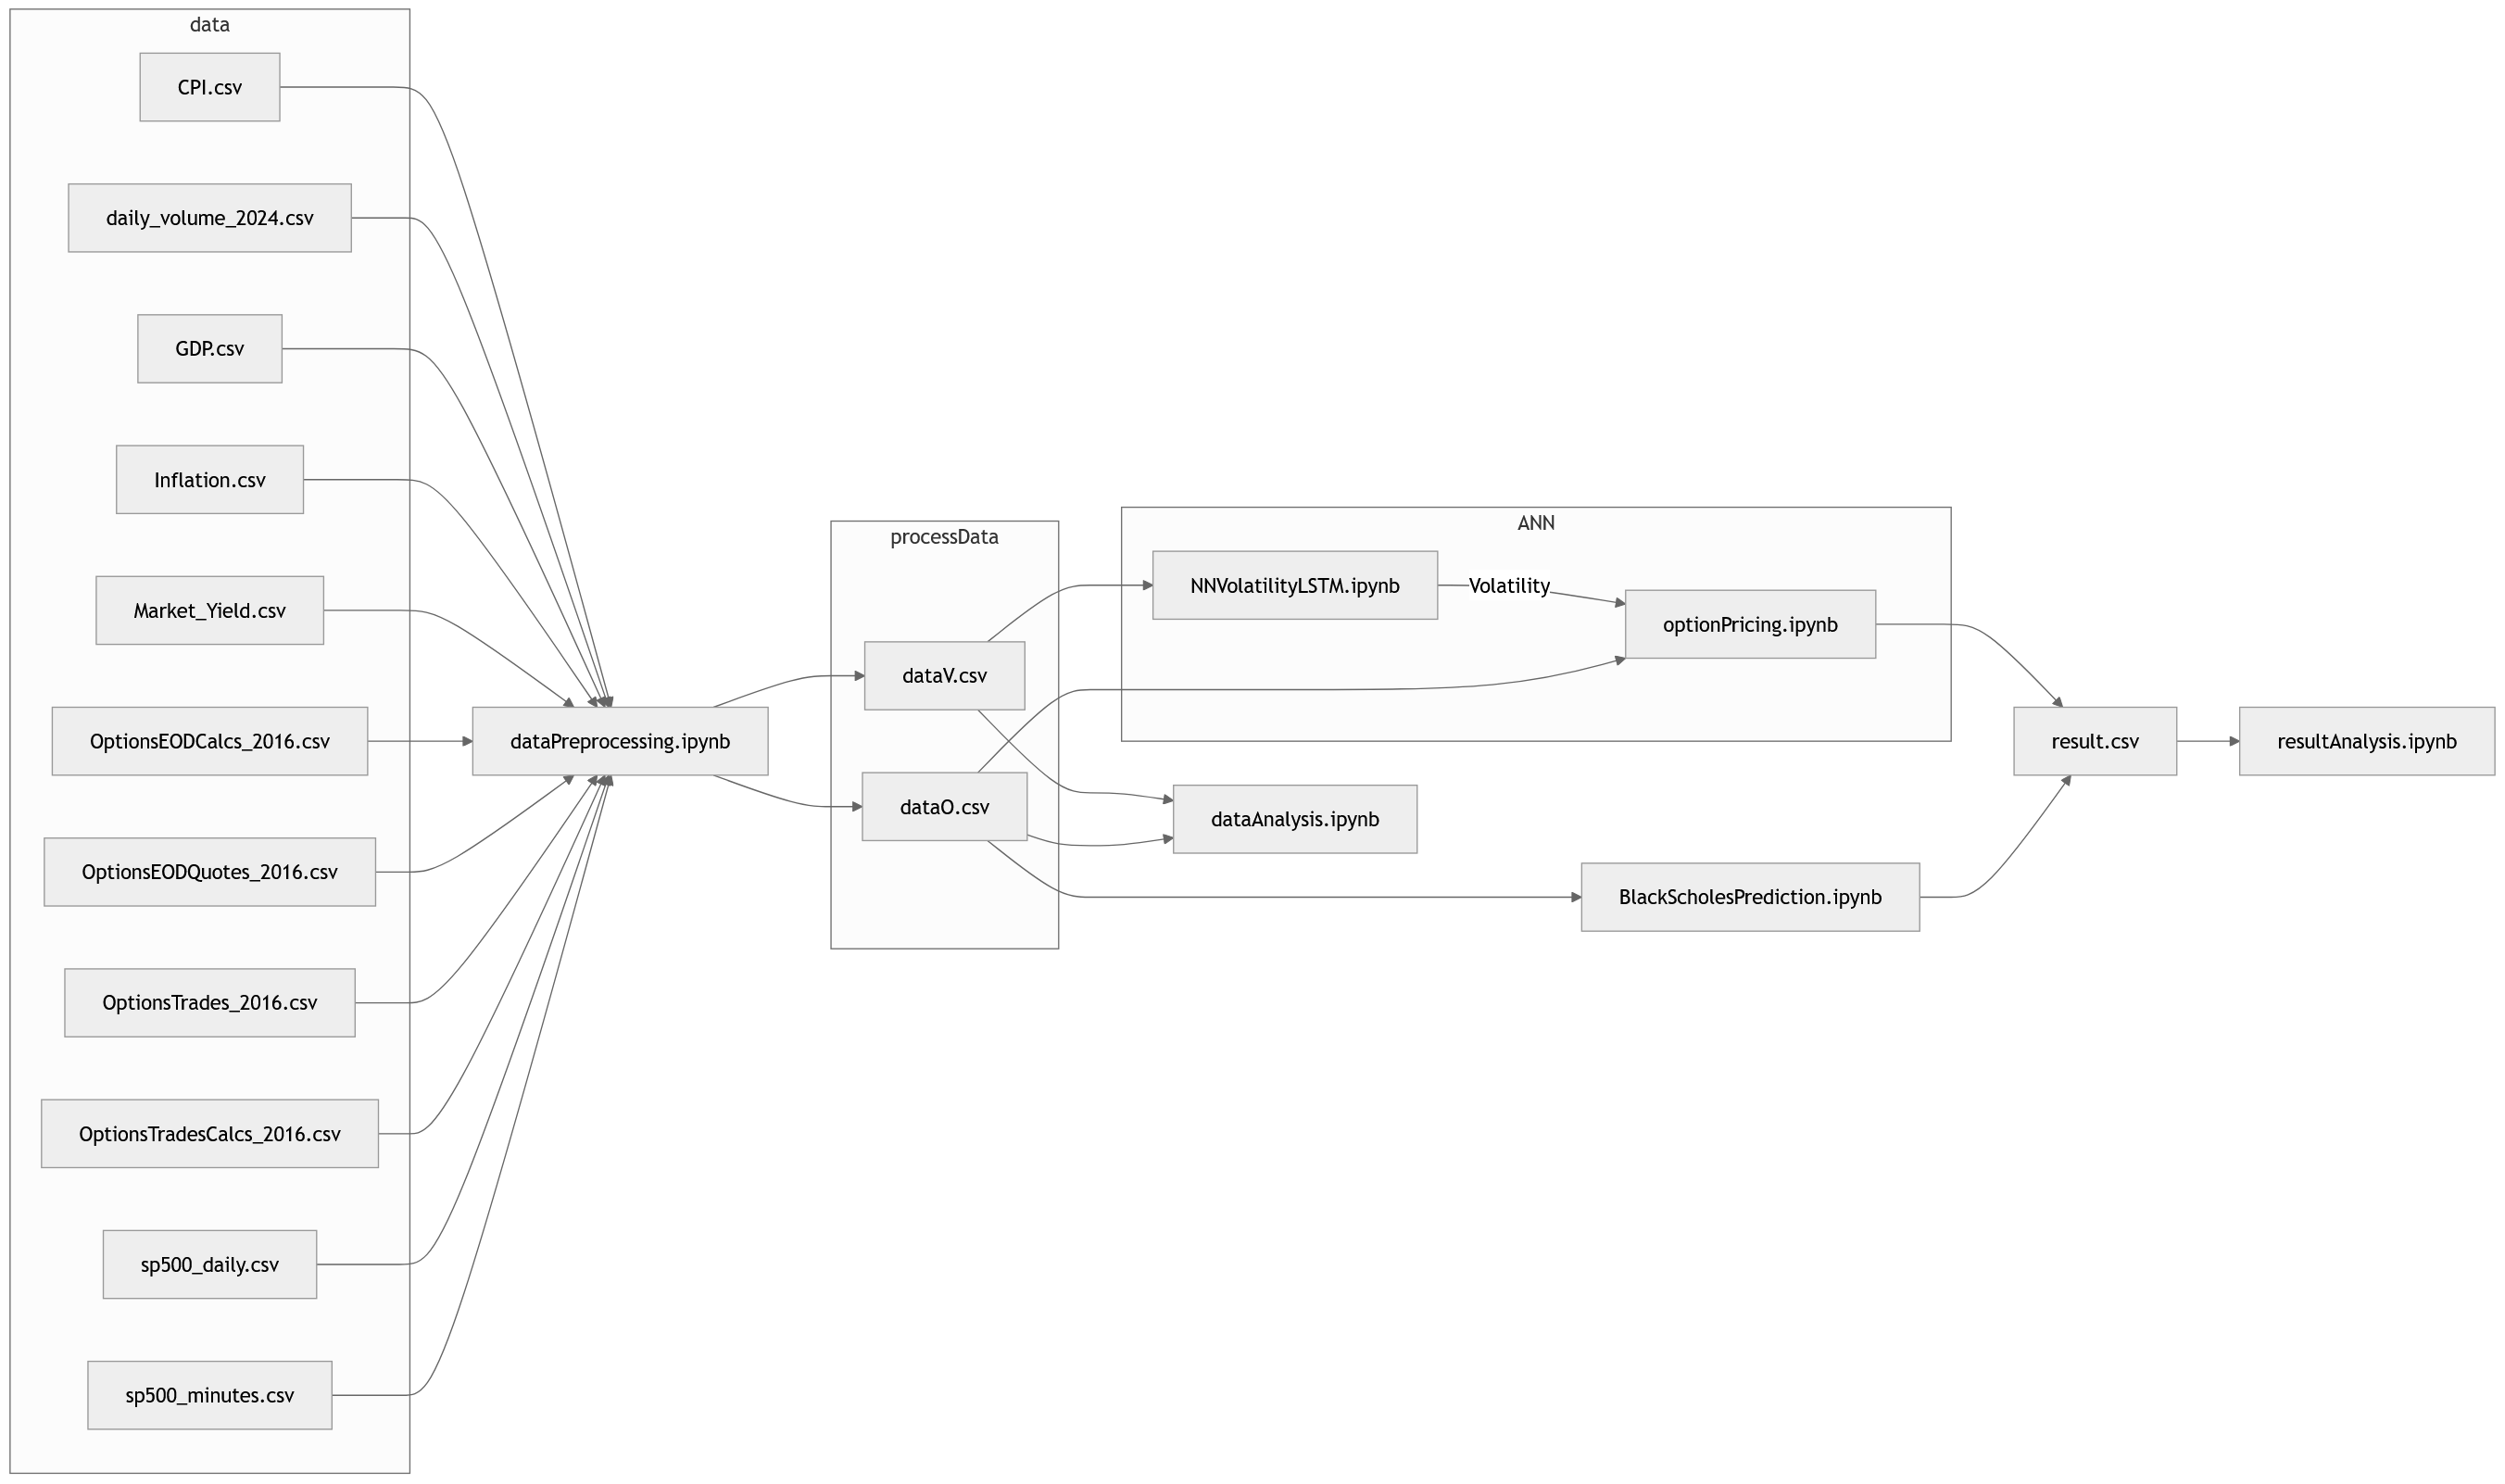
\includegraphics[width=0.9\textwidth]{img/structure.png}
            \end{center}

\newpage
\section*{Iteration 1}
\begin{flushright}
February 3, 2025
\end{flushright}
\hrule
\vspace{0.2in}

\subsection*{What Is New?}
\begin{itemize}
    \item Created and trained a model for option pricing, using Black-Scholes parameters to target option prices.
            
\begin{figure}[H]
  \centering
  \begin{minipage}[b]{0.45\textwidth}
    \centering
    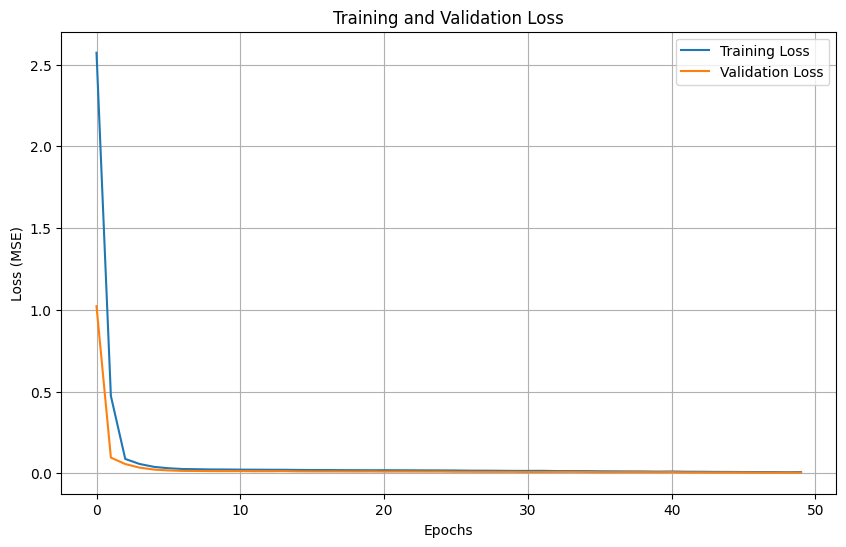
\includegraphics[width=\linewidth]{img/Loss_options_model.png} 
  \end{minipage}
  \hfill
  \begin{minipage}[b]{0.5\textwidth}
    \centering
    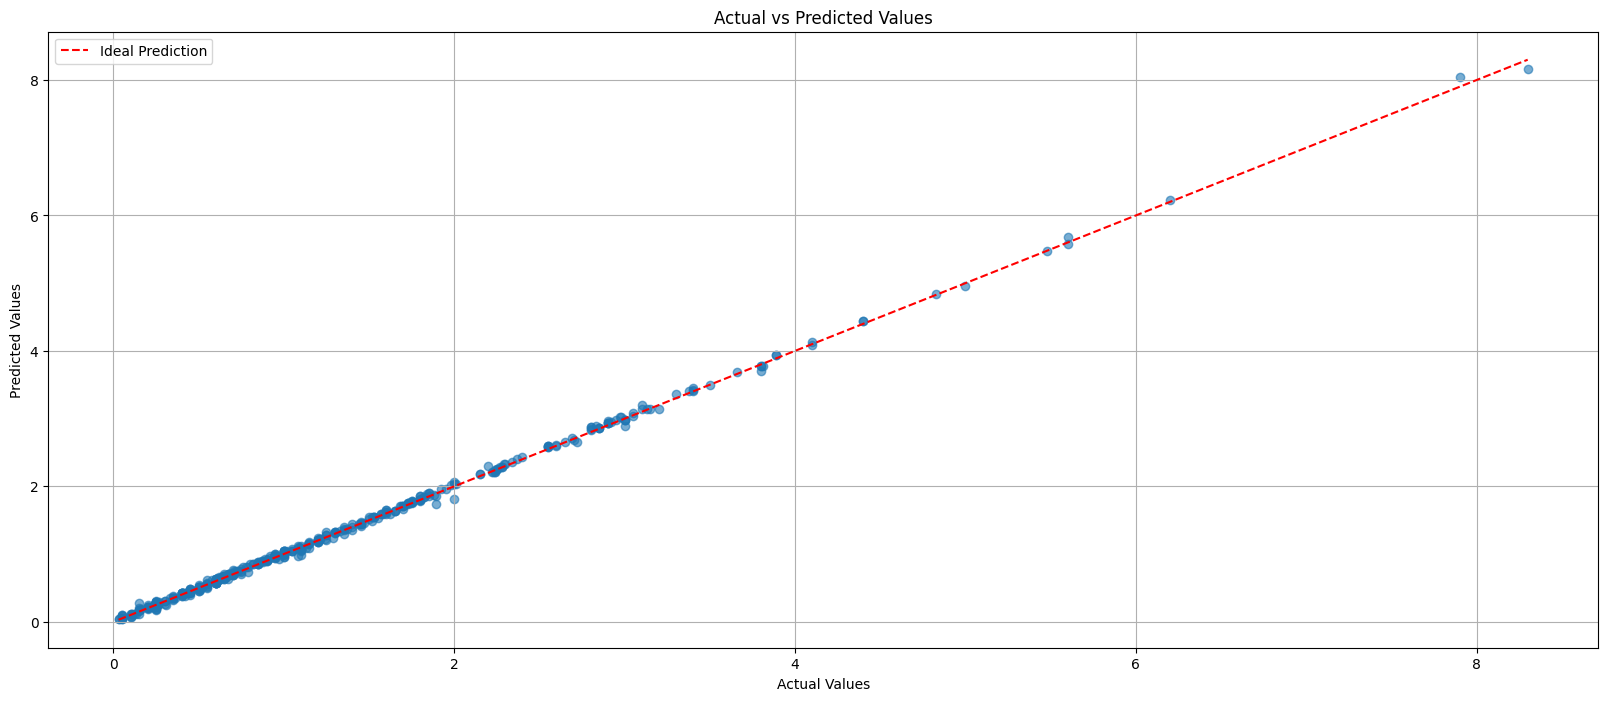
\includegraphics[width=\linewidth]{img/OPMreg.png}
  \end{minipage}
\end{figure}

    \item Compared the model's performance against Black-Scholes models:
            \begin{center}
            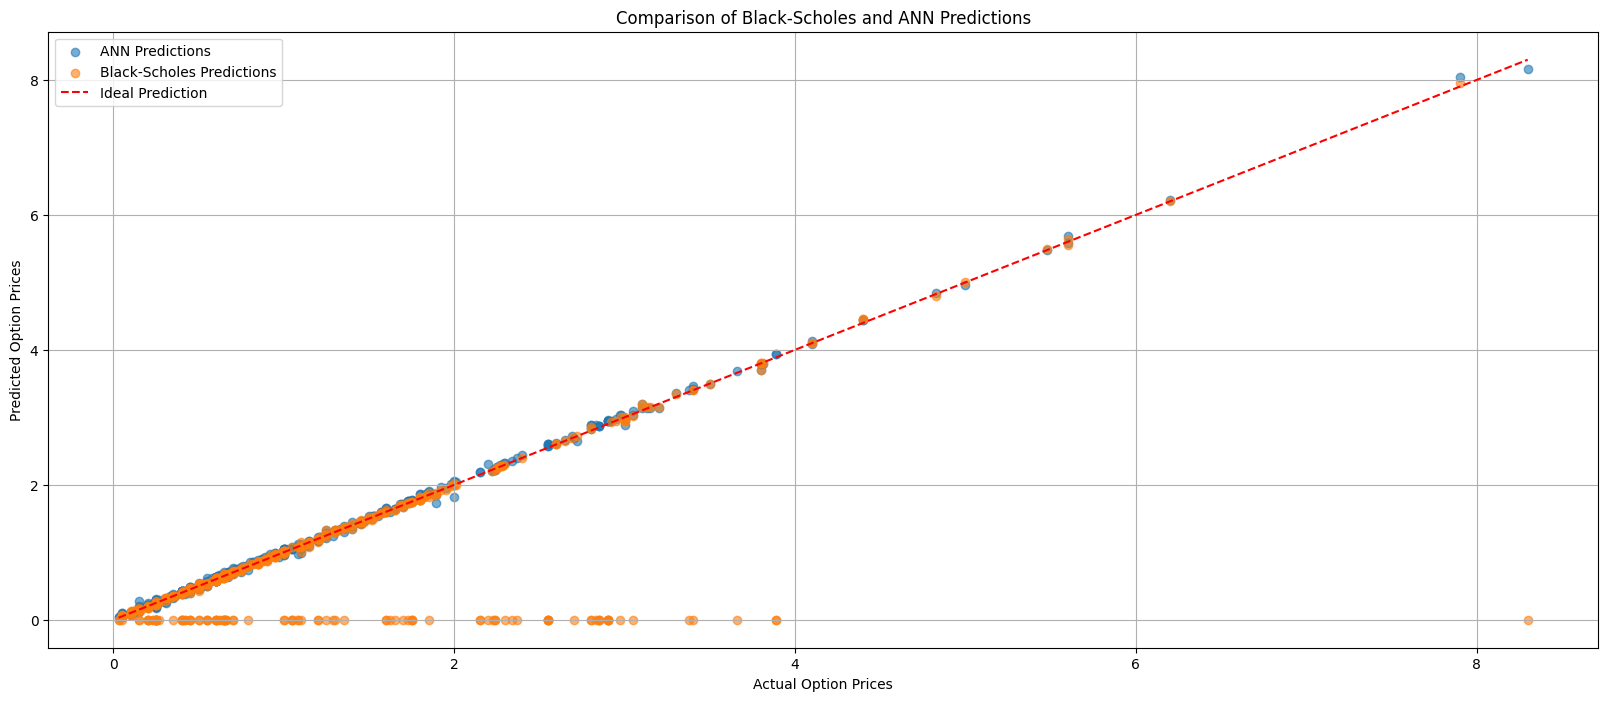
\includegraphics[width=0.8\textwidth]{img/BSvANN.png}
            \end{center}
            
    \item Started to build a custom LSTM model with NumPy. For now, I think Python allows better flexibility and development time than C++, while still maintaining decent performance using only NumPy. 
    I want the model to be compatible with TensorFlow formatting for easier use. It can be found in \href{https://github.com/PaulAnrd/Research_Project}{code/models/annModels.py}.
\end{itemize}

\subsection*{What Is Next?}
\begin{itemize}
    \item Finish the custom model.
\end{itemize}

\end{document}
